\chapter{Suggestions to Improve The Existing System} \label{suggestions}

\section{System Perspective}

\begin{figure}[H]
  \centering
  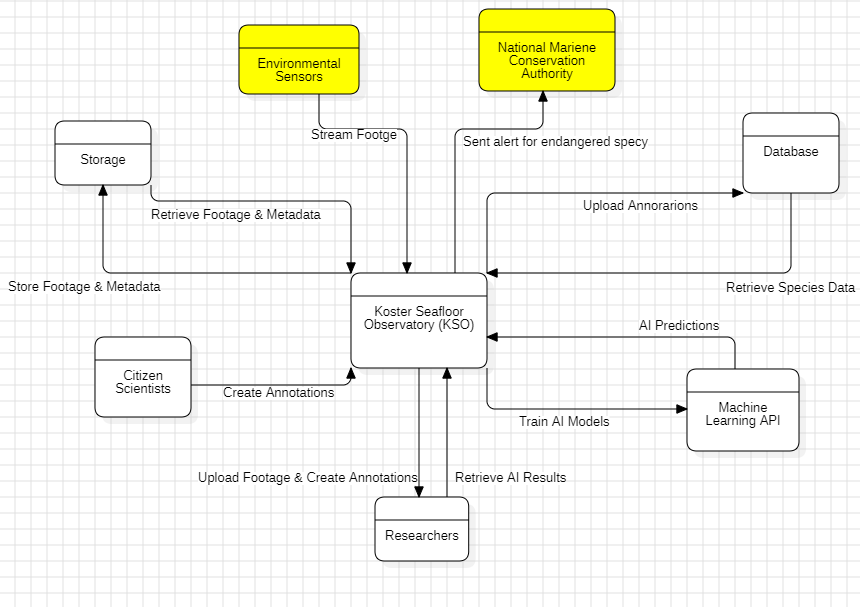
\includegraphics[width=1 \textwidth]{Figures/ImpSystem Context Diagram.png}
  \caption{Improved System Context Diagram \label{Fig:Improved System Context Diagram}}
\end{figure}

\paragraph{Environmental Sensors (Video Stream for Live Detection):}
Environmental sensors integrated within the KSO platform provide continuous subsea video streams, facilitating real-time detection and identification of marine species via AI-driven models. This integration significantly enhances biodiversity assessments and supports immediate ecological analysis and decision-making.

\paragraph{National Marine Conservation Authority (Alerts for Extinct Species):}
The KSO system automatically issues instantaneous alerts to the National Marine Conservation Authority upon the detection of extinct or critically endangered marine species. This proactive alert mechanism ensures rapid conservation responses and timely protection measures for vulnerable marine biodiversity.

\section{External Interfaces}

\begin{figure}[H]
  \centering
  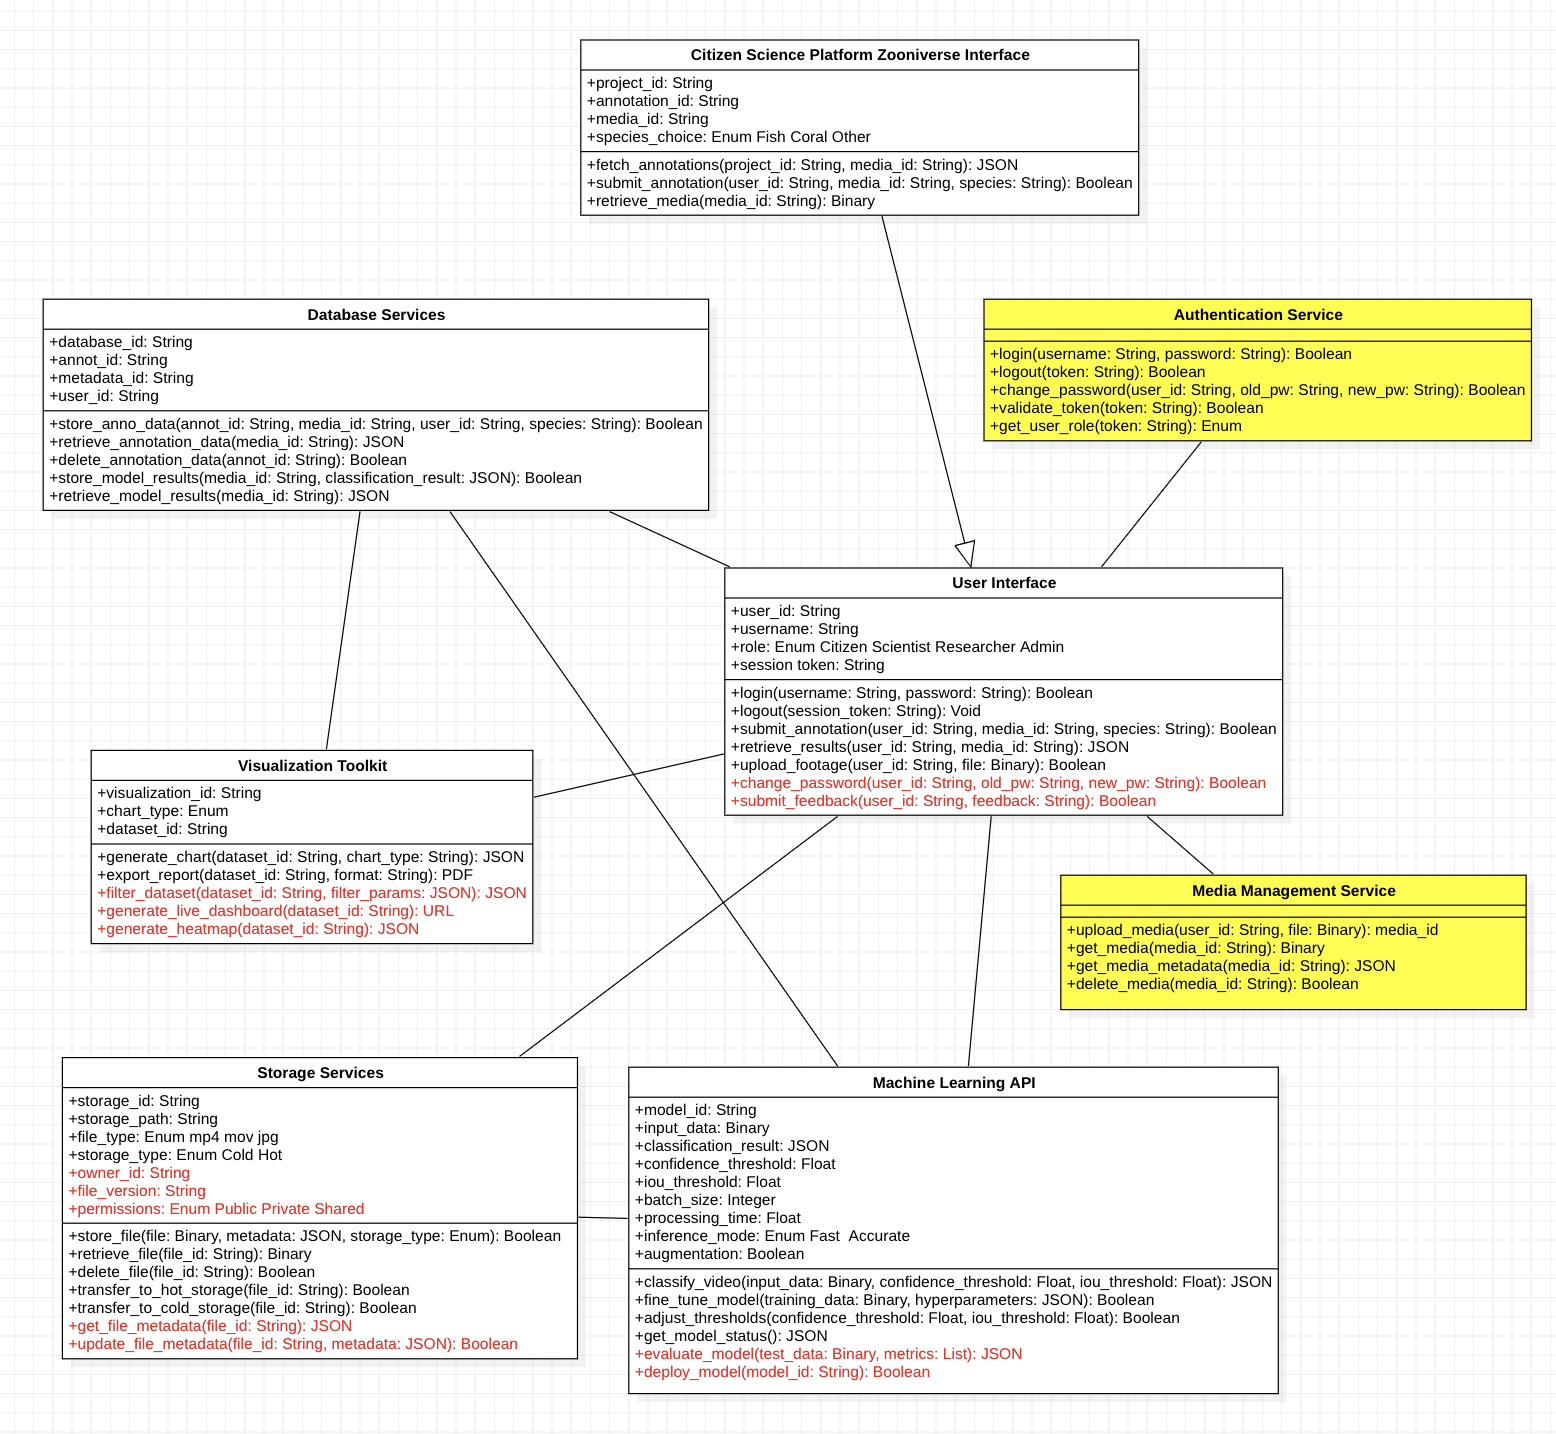
\includegraphics[width=0.98 \textwidth]{Figures/ImpExternalInterfaces.png}
  \caption{Improved External Interfaces Diagram \label{Fig:Improved System Context Diagram}}
\end{figure}

\paragraph{}
The \textbf{Authentication Service} has been added in order to isolate the login, logout, and token validation logic for users from the \textbf{User Interface} class. It is an example of the use of the principle of separation of concerns and makes authentication safe for reuse by other components like APIs and background services. Centralization of session handling, role authentication, and token verification makes the system scalable, testable, and maintainable.

The \textbf{Media Management Service} was introduced to centralize media operations such as uploading, retrieval, deletion, and accessing metadata. Media management in the current design is scattered between the \textbf{User Interface} and \textbf{Zooniverse} classes, leading to duplication and unbalanced logic. A standalone media manager offers better control, clearer responsibilities, and flexibility to deal with different file types, metadata, and storage levels across the system.

The \textbf{Machine Learning API} was also supplemented with model evaluation and deployment. These are genuine requirements in practical ML systems in which models have to be retrained, tested, monitored, and deployed in incremental steps. With fine-tuning, deployment, and monitoring of status enabled, the API is an end-to-end ML lifecycle manager enabling continuous improvement and good automation.

The \textbf{Visualization Toolkit} was enhanced to support filtering, real-time dashboards, heatmap generation, and export in multiple formats. These improvements empower users and researchers to extract more meaningful insights from their data and reports. By enabling dynamic interaction with datasets, the toolkit becomes a powerful interface for data exploration, which is especially valuable in citizen science and research-oriented platforms like KSO.

\textbf{Storage Services} were also improved to enable metadata access, file versioning, permissions, and user-based file listings. The upgrade enables support for handling higher volumes of data more effectively with fine-grained control over file ownership, visibility, and lifecycle. These features are aligned with cloud storage best practices and are required to offer secure, multi-user environments.

\section{Functions}
\begin{figure}[H]
  \centering
  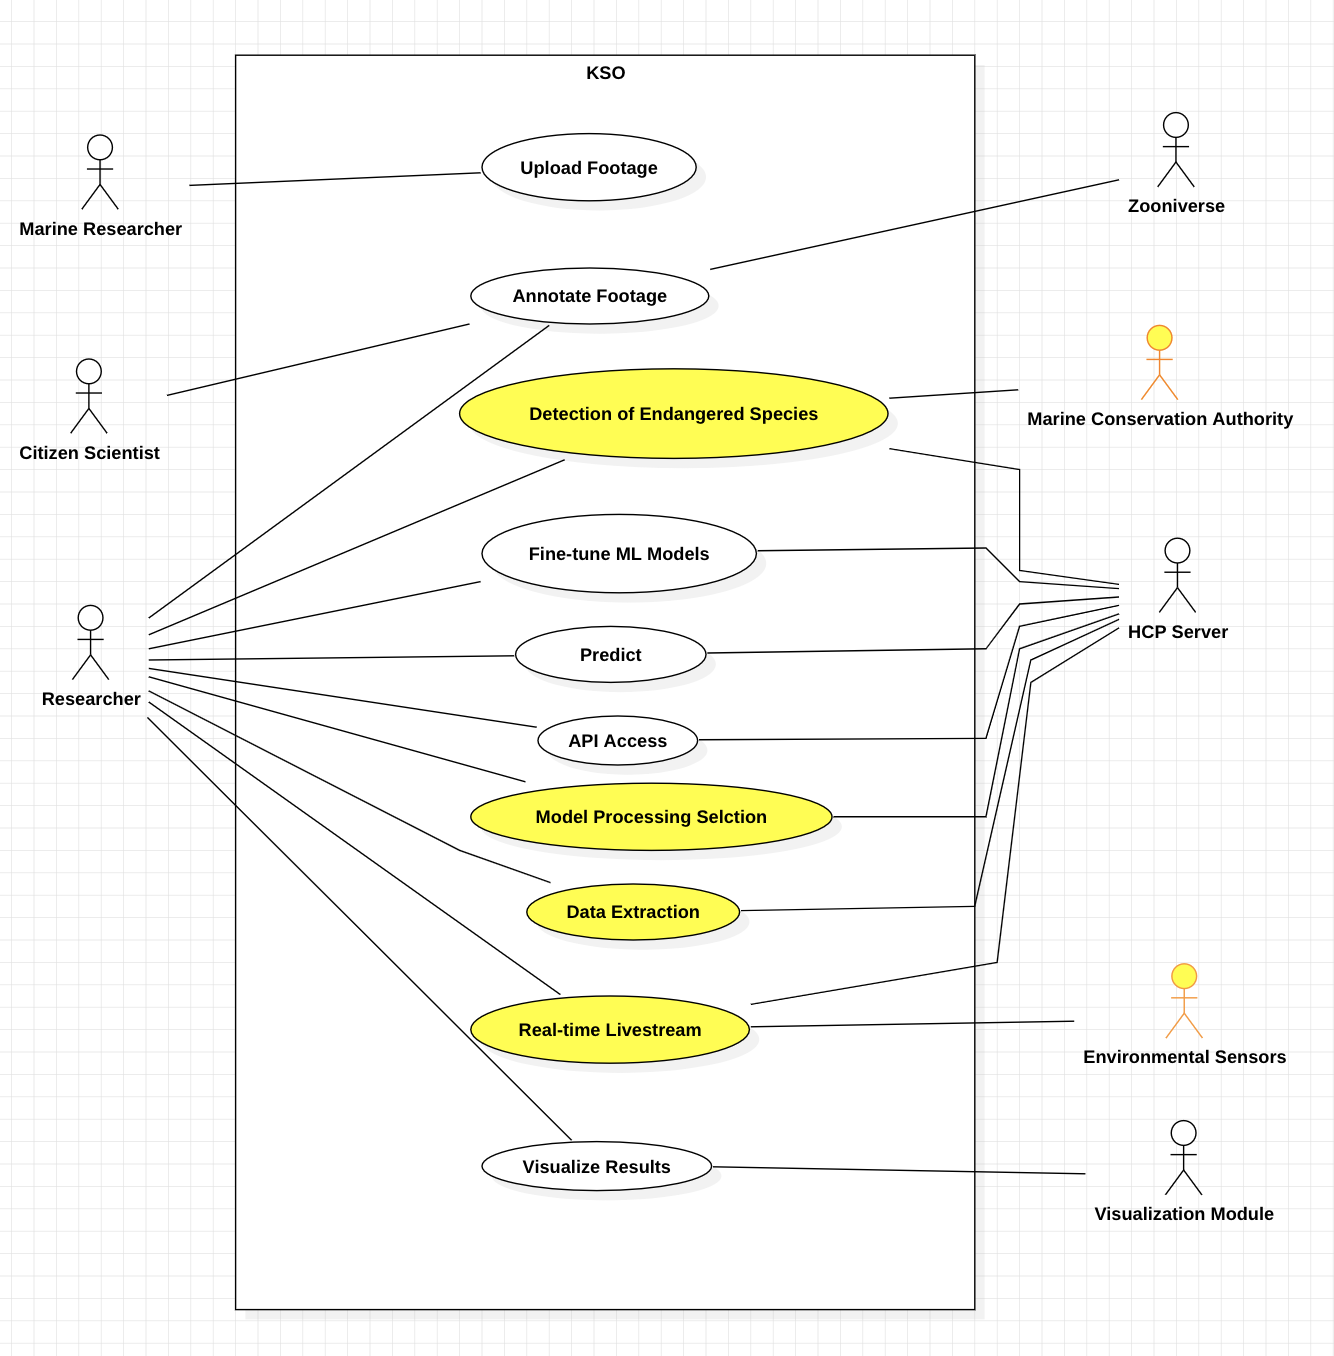
\includegraphics[width=1 \textwidth]{Figures/ImpUseCase Diagram.png}
  \caption{Improved UseCase Diagram \label{Fig:Improved UseCase Diagram}}
\end{figure}


\begin{table}[H] 
  \centering
  \footnotesize
  \begin{tabularx}{\textwidth}{|>{\bfseries\hsize=.5\hsize\linewidth=\hsize}X|
  >{\hsize=1.5\hsize\linewidth=\hsize}X|}
  \hline
  Use Case Name       & Detection of Endangered or Possibly Extinct Marine Species \\ \hline
  
  Actors              & HPC Server, Researcher, Marine Conservation Authority \\ \hline
  
  Description         & The system detects rare species in multiple frames and alerts researchers and conservation authorities. \\ \hline
  
  Pre-Conditions      & 
  - Species detected in multiple frames.\newline
  - Confidence score should be higher than 90\%.\newline
  - Species exists in endangered/extinct sea creatures database.\newline
  - Conservation authority contact available. \\ \hline
  
  Data                & 
  - Species name, confidence score, coordinates, timestamp, video frame.\newline
  - Historical records (if available). \\ \hline
  
  Response            & 
  - System flags detection and notifies researcher.\newline
  - If verified, an alert is sent to the authority. \\ \hline
  
  Stimulus            & ML model detects an endangered or extinct species across multiple frames. \\ \hline
  
  Normal Flow         & 
  1. System processes video and detects species.\newline
  2. Checks confidence level and number of frames.\newline
  3. Cross-references with species database.\newline
  4. If valid, flags detection and notifies researcher.\newline
  5. Researcher verifies detection.\newline
  6. If confirmed, system alerts conservation authority. \\ \hline
  
  Alternative Flow    & If researcher finds an error, detection is discarded and model is adjusted. \\ \hline
  
  Exception Flow      & 
  - If confidence is lower than 90\%, system requests further verification.\newline
  - If no authority response, system retries later. \\ \hline
  
  Post-Conditions     & 
  - Verified sightings logged in biodiversity records.\newline
  - Data supports conservation actions. \\ \hline
  
  Comments            & 
  - Ensures high accuracy by requiring multiple frame detections.\newline
  - Supports real-time conservation efforts. \\ \hline
  \end{tabularx}
  \caption{Tabular Description of \textit{Detection of Endangered or Possibly Extinct Marine Species} }
  \label{Tab:UseCase3}
\end{table}

\begin{figure}[H]
  \centering
  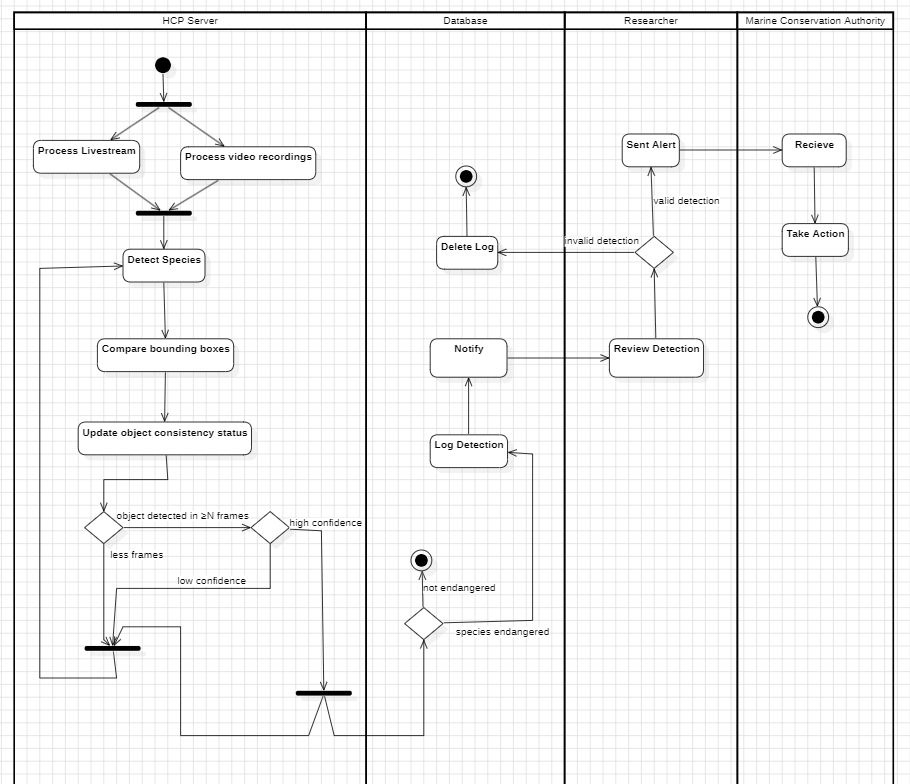
\includegraphics[width=1.1 \textwidth]{Figures/ImpActivity Diagram.png}
  \caption{Activity Diagram of Detection of Endangered or Possibly Extinct Marine Species \label{Fig:Improved Activity Diagram}}
\end{figure}

\begin{table}[H] 
  \centering
  \footnotesize
  \begin{tabularx}{\textwidth}{|>{\bfseries\hsize=.5\hsize\linewidth=\hsize}X|
  >{\hsize=1.5\hsize\linewidth=\hsize}X|}
  \hline
  Use Case Name       & Real-Time Marine Monitoring via Livestream and Environmental Sensors \\ \hline
  
  Actors              & Environmental Sensors, Researcher, HPC Server \\ \hline
  
  Description         & The system processes livestream footage and environmental data to monitor marine life in real time. \\ \hline
  
  Pre-Conditions      & 
  - Livestream cameras and environmental sensors are active.\newline
  - AI model processes incoming frames.\newline
  - Internet connectivity is stable. \\ \hline
  
  Data                & 
  - Video stream data, detected species, confidence score.\newline
  - Environmental parameters (temperature, pH, oxygen levels, salinity). \\ \hline
  
  Response            & 
  - System displays detected species in real-time.\newline
  - Researchers receive notifications of notable detections.\newline
  - Environmental changes are logged and analyzed. \\ \hline
  
  Stimulus            & The system receives continuous livestream and sensor data. \\ \hline
  
  Normal Flow         & 
  1. System continuously processes livestream footage.\newline
  2. AI detects marine species and classifies them in real time.\newline
  3. System overlays detection data on the live feed.\newline
  4. Environmental sensor data is correlated with detected species.\newline
  5. Users view real-time species identification through an interactive dashboard.\newline
  6. System logs detections and environmental conditions for further analysis. \\ \hline
  
  Alternative Flow    & 
  - If AI confidence is low, system requests additional frames before confirming detection.\newline
  - If no species is detected, system continues monitoring without notifications. \\ \hline
  
  Exception Flow      & 
  - If livestream connectivity fails, system retries connection.\newline
  - If environmental sensors provide anomalous readings, system alerts researchers. \\ \hline
  
  Post-Conditions     & 
  - Detected species and environmental data are logged.\newline
  - Users and researchers gain real-time insights into marine biodiversity. \\ \hline
  
  Comments            & 
  - Enables real-time marine life monitoring for research and conservation.\newline
  - Can be integrated with public educational platforms for citizen science. \\ \hline
  \end{tabularx}
  \caption{Tabular Description of \textit{Real-Time Marine Monitoring via Livestream and Environmental Sensors} }
  \label{Tab:UseCaseLivestream}
\end{table}

\begin{figure}[H]
  \centering
  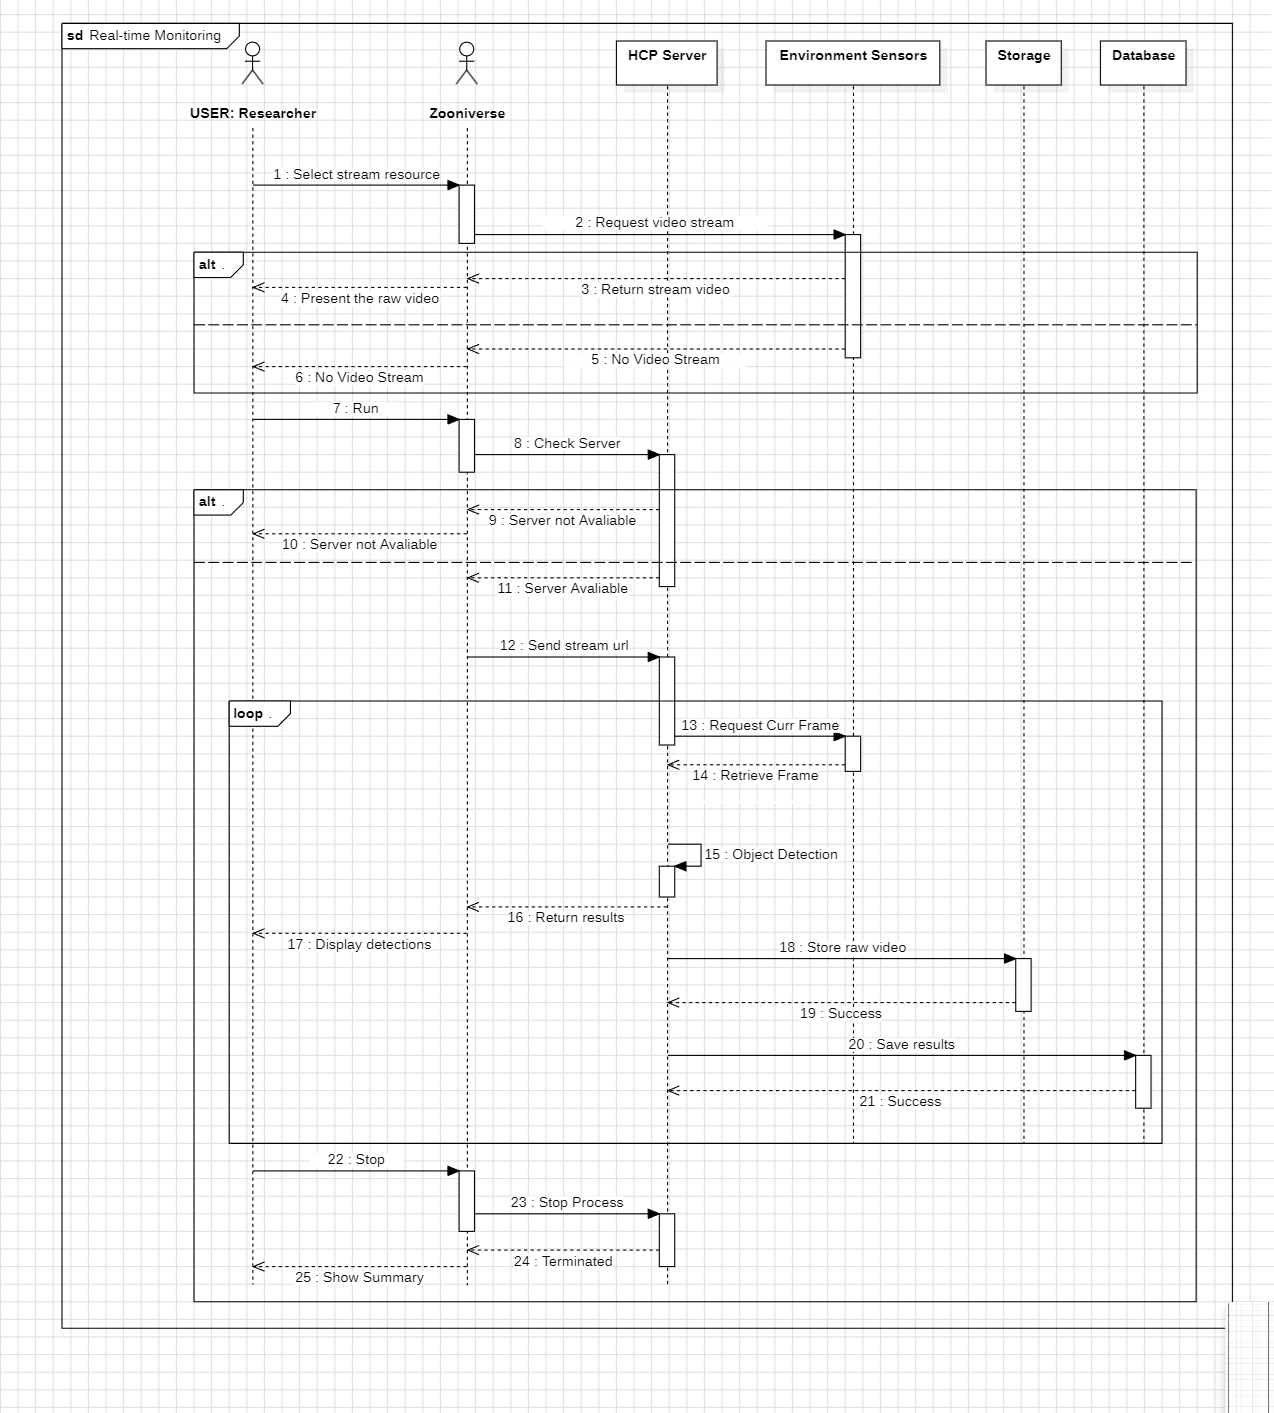
\includegraphics[width=1 \textwidth]{Figures/ImpSequence Diagram.png}
  \caption{Sequence Diagram of Real-Time Marine Monitoring via Livestream and Environmental Sensors \label{Fig:Improved Sequence Diagram}}
\end{figure}

\begin{table}[H] 
  \centering
  \footnotesize
  \begin{tabularx}{\textwidth}{|>{\bfseries\hsize=.5\hsize\linewidth=\hsize}X|
  >{\hsize=1.5\hsize\linewidth=\hsize}X|}
  \hline
  Use Case Name       & Model Processing Selection: GPU vs. TPU \\ \hline
  
  Actors              & Researcher, HCP Server \\ \hline
  
  Description         & Users can choose between GPU and TPU for model execution, with TPU usage limited by available credits. \\ \hline
  
  Pre-Conditions      & 
  - The system has access to both GPU and TPU resources.\newline
  - TPU credits are available.\newline
  - User has the appropriate permissions to select hardware. \\ \hline
  
  Data                & 
  - User’s hardware selection (GPU/TPU).\newline
  - Remaining TPU credits.\newline
  - Model processing time and resource usage logs. \\ \hline
  
  Response            & 
  - The system runs the model on the selected hardware.\newline
  - TPU credits are deducted if TPU is used.\newline
  - System notifies the user if credits are insufficient. \\ \hline
  
  Stimulus            & User selects model execution hardware (GPU or TPU). \\ \hline
  
  Normal Flow         & 
  1. User accesses model execution settings.\newline
  2. User selects GPU (default) or TPU for processing.\newline
  3. System checks TPU credit balance.\newline
  4. If credits are sufficient, TPU execution starts, and credits are deducted.\newline
  5. If GPU is selected, the model runs without restrictions.\newline
  6. System processes the model and returns results.\newline
  7. Usage is logged for performance tracking. \\ \hline
  
  Alternative Flow    & 
  - If TPU credits are low, system suggests switching to GPU or allows the user to purchase additional credits.\newline
  - If TPU is at capacity, system queues the job or offers a GPU alternative. \\ \hline
  
  Exception Flow      & 
  - If TPU execution fails, the system falls back to GPU processing.\newline
  - If the GPU is overloaded, the system suggests scheduling the job later. \\ \hline
  
  Post-Conditions     & 
  - Model execution completes on the selected hardware.\newline
  - TPU credits are updated if used.\newline
  - Execution logs are stored for tracking and optimization. \\ \hline
  
  Comments            & 
  - Similar to Google Colab, allowing flexible TPU/GPU selection.\newline
  - Ensures efficient resource allocation based on availability and user needs. \\ \hline
  \end{tabularx}
  \caption{Tabular Description of \textit{Model Processing Selection: GPU vs. TPU} }
  \label{Tab:UseCaseHardwareSelection}
\end{table}

\begin{figure}[H]
  \centering
  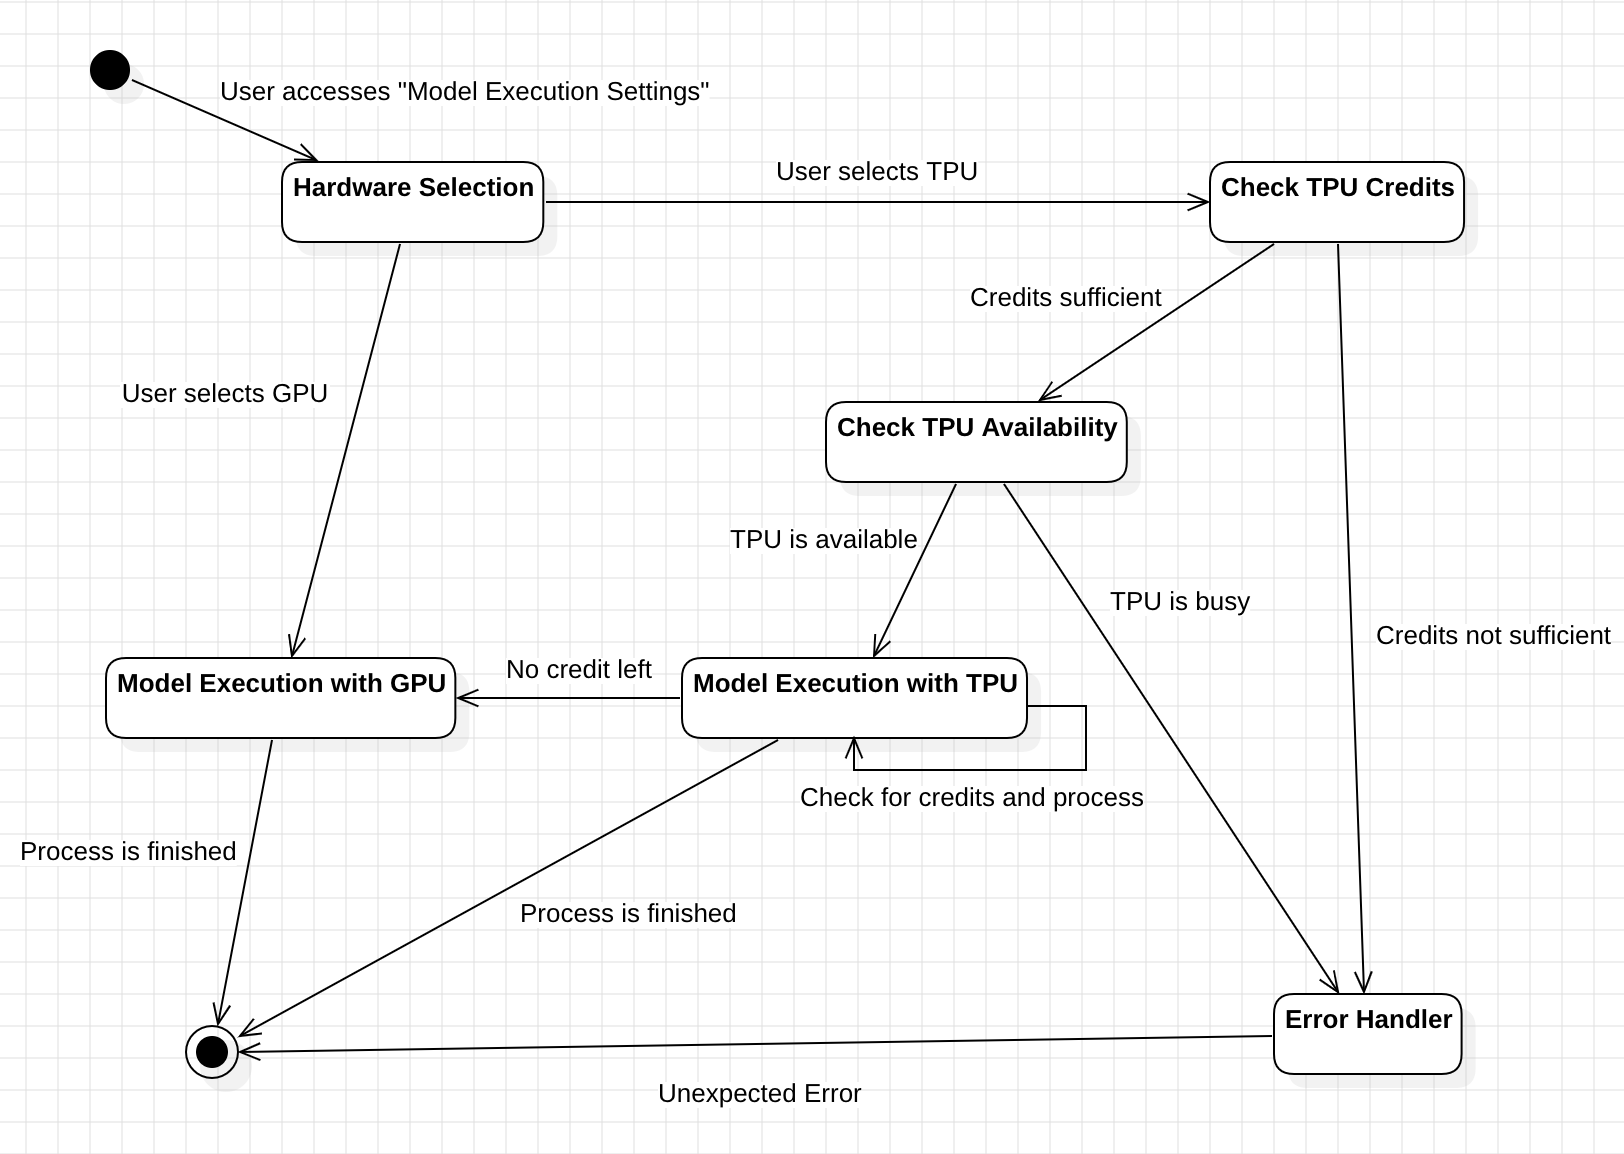
\includegraphics[width=1 \textwidth]{Figures/GpuTpuStateDiagram.png}
  \caption{State Diagram of Model Processing Selection: GPU vs. TPU \label{Fig:Improved System Context Diagram}}
\end{figure}

\begin{table}[H] 
  \centering
  \small
  \begin{tabularx}{\textwidth}{|>{\bfseries\hsize=.5\hsize\linewidth=\hsize}X|
  >{\hsize=1.5\hsize\linewidth=\hsize}X|}
  \hline
  Use Case Name       & Data Extraction for Researchers \\ \hline
  
  Actors              & HPC Server, Researcher \\ \hline
  
  Description         & Researchers can extract processed biodiversity and environmental data for analysis and reporting. \\ \hline
  
  Pre-Conditions      & 
  - The researcher has access to the system.\newline
  - Required data (species detections, environmental readings) is available in the database.\newline
  - User has permissions for data export. \\ \hline
  
  Data                & 
  - Species detection records (location, time, confidence score).\newline
  - Environmental sensor data (temperature, pH, oxygen levels, etc.).\newline
  - Model predictions and annotations.\newline
  - Export format selection (CSV, JSON, API). \\ \hline
  
  Response            & 
  - HPC Server generates and provides the requested dataset.\newline
  - Large datasets may be compressed before download.\newline
  - API users receive structured data responses. \\ \hline
  
  Stimulus            & Researcher requests a data extraction. \\ \hline
  
  Normal Flow         & 
  1. Researcher logs into the system.\newline
  2. Researcher selects desired data type and time range.\newline
  3. HPC Server retrieves requested records from the database.\newline
  4. Researcher chooses export format (CSV, JSON, API response).\newline
  5. HPC Server processes the extraction request.\newline
  6. Data is provided for download or accessed via API.\newline
  7. Extraction log is recorded. \\ \hline
  
  Alternative Flow    & 
  - If dataset is large, system notifies user about processing time.\newline
  - If multiple formats are needed, system allows batch export. \\ \hline
  
  Exception Flow      & 
  - If no matching data is found, system notifies researcher.\newline
  - If database is under maintenance, system queues the request. \\ \hline
  
  Post-Conditions     & 
  - Extracted data is available for further research.\newline
  - System logs the extraction for tracking purposes. \\ \hline
  
  Comments            & 
  - Supports biodiversity research and marine conservation analysis.\newline
  - API access allows integration with external research tools. \\ \hline
  \end{tabularx}
  \caption{Tabular Description of \textit{Data Extraction for Researchers} }
  \label{Tab:UseCaseDataExtraction}
\end{table}

\section{Logical Database Requirements}

\begin{figure}[H]
    \centering
    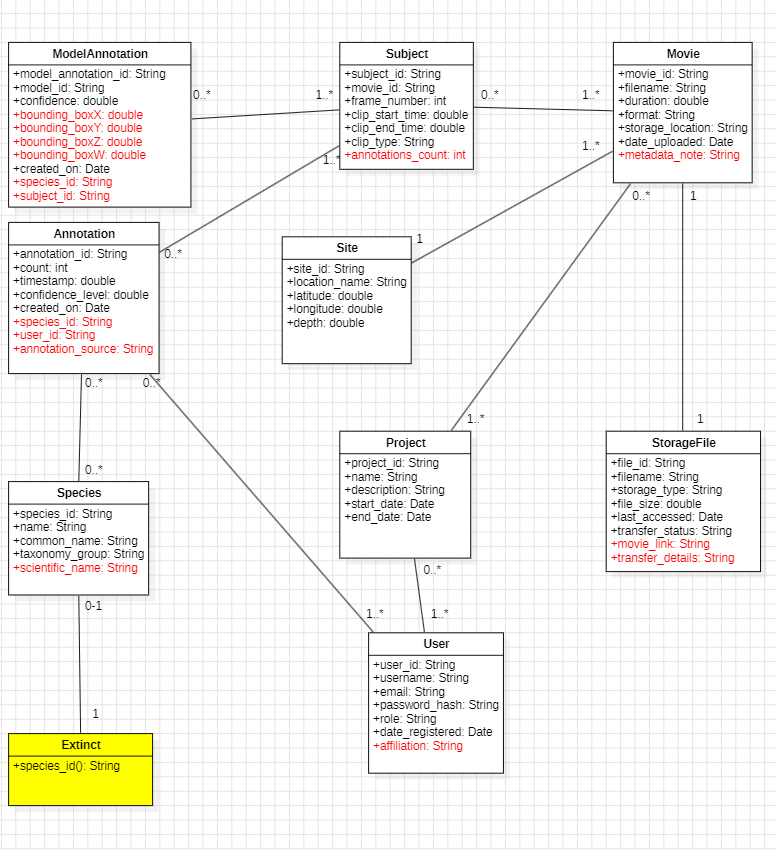
\includegraphics[width=1 \textwidth]{Figures/ImpLogicalDatabase.png}
    \caption{Improved Logical Database Diagram \label{Fig:Improved Logical Database Diagram}}
\end{figure}


\paragraph{} 
We introduced several new fields to enhance clarity and flexibility: 
\texttt{species\_id} and \texttt{scientific\_name} provide consistent 
references for each annotated organism, while \texttt{user\_id} and 
\texttt{annotation\_source} distinguish who or what created each 
annotation (e.g.\ expert, citizen scientist, or AI). By adding 
\texttt{subject\_id}, we ensure annotations align precisely with specific 
clips or frames, and \texttt{bounding\_box\_coordinates} captures the 
exact location of the detected species within an image. To store additional 
context, we included \texttt{metadata\_note} in our media records, and 
for user profiles, we added \texttt{affiliation} to track organizational 
or institutional ties. Additionally, to support monitoring and rapid 
conservation alerts, we introduced a new table, \texttt{Extinct}, which 
references the \texttt{species\_id} as a foreign key, clearly identifying 
species marked as extinct or critically endangered.



\section{System Quality Attributes}

\subsection{Suggestions to Improve Usability Requirements}
\begin{itemize}
    \item \textbf{Guided Tutorials:} Integrate short, interactive video or text-based tutorials tailored to first-time users, helping them understand annotation protocols and platform features more quickly.
    \item \textbf{Adaptive Interface:} Consider adding user-level adaptability to display simpler or more complex features based on user proficiency, thus accommodating both novice and expert contributors.
\end{itemize}

\subsection{Suggestions to Improve Performance Requirements}
\begin{itemize}
    \item \textbf{Cache Mechanisms:} Implement caching strategies for repeated video access and model predictions to reduce redundant computations and accelerate load times.
    \item \textbf{Parallel Data Processing:} Adopt parallel processing or distributed computing for resource-intensive tasks such as large-scale video conversions or batch inference jobs, making full use of modern HPC architectures.
    \item \textbf{Scalability Testing:} Periodically perform stress tests to identify bottlenecks under high user load or large data volumes; these tests help guide hardware upgrades or optimizations in system architecture.
\end{itemize}

\subsection{Suggestions to Improve Reliability Requirements}
\begin{itemize}
    \item \textbf{Redundant Backups:} Schedule automated backups of both raw video and annotated data to off-site or cloud storage to mitigate data loss risks.
    \item \textbf{Health Monitoring:} Implement monitoring tools (e.g., Prometheus, Grafana) to track system metrics and quickly identify anomalies or potential failures.
    \item \textbf{Failover Strategy:} Define procedures to switch to backup systems or mirror databases in the event of primary component failure, minimizing downtime for users.
\end{itemize}

\subsection{Suggestions to Improve Maintainability Requirements}
\begin{itemize}
    \item \textbf{Modular Code Reviews:} Implement a peer review process where each module is reviewed by multiple developers, ensuring code quality and knowledge sharing.
    \item \textbf{Design Patterns and Best Practices:} Standardize architectures (e.g., microservices) and coding guidelines to ensure consistent implementations across modules.
\end{itemize}

\subsection{Suggestions to Improve Portability Requirements}
\begin{itemize}
    \item \textbf{Containerization:} Package core components (database, web front-end, machine learning services) in containers (e.g., Docker) to streamline deployments across multiple environments.
    \item \textbf{Cross-Browser Testing:} Continuously validate that the interface renders correctly on major web browsers (e.g., Chrome, Firefox, Safari, Edge) to avoid unexpected UI/UX issues.
    \item \textbf{Adaptive UI Design:} Ensure the front-end is responsive and supports diverse screen resolutions, enabling efficient use on tablets, smartphones, and various display sizes.
\end{itemize}

\section{Design Constraints}

\begin{enumerate}
    \item \textbf{Enhanced Standards Compliance and Data Interoperability}
      \begin{itemize}
        \item \textbf{Adopt Additional Metadata Standards:} In addition to Darwin Core (DwC), we can incorporate widely used schemas (e.g., ABCD, MIxS) or extend DwC fields to capture more granular information (e.g., habitat type, light levels, or ROV operational details). This promotes seamless integration with other marine datasets and expands future analytical potential.
        \item \textbf{Strengthen Versioning Protocols:} Implement version-control systems for both raw and annotated datasets to ensure provenance is fully traceable. Maintaining a structured change log will allow researchers to track and cite specific data revisions confidently.
      \end{itemize}
  
    \item \textbf{Open-Source Software and Reproducibility}
      \begin{itemize}
        \item \textbf{Adopt a Community-Driven Development Model:} Encourage external contributions to core modules (e.g., machine learning pipelines, data ingestion scripts) by using a transparent governance approach such as Requests for Comment (RFC) on public code repositories. This fosters a broader support network and quicker integration of cutting-edge methods.
      \end{itemize}
  
    \item \textbf{Strengthened Ethical and Regulatory Compliance}
      \begin{itemize}
        \item \textbf{Automate Compliance Checks:} Integrate compliance audits (GDPR, Zooniverse terms) into the development pipeline. For example, script-based checks can verify that no personal data is stored, that consent is properly documented, and that data usage remains within ethical guidelines.
        \item \textbf{Incorporate Accessibility Standards:} Ensure the citizen science interface follows accessibility guidelines (e.g., WCAG 2.1). This broadens volunteer inclusivity and may be required by funders and institutions advocating for accessible digital environments.
      \end{itemize}
  
    \item \textbf{Future-Proofing Hardware and Computational Constraints}
      \begin{itemize}
        \item \textbf{Design for Scalable Architecture:} Although current GPU and CPU resources may be sufficient, plan for seamless scaling to larger or distributed clusters if future data volumes or model complexity outgrow on-site capacity. Containerization (e.g., Docker, Kubernetes) can facilitate portability and load balancing across multiple machines.
        \item \textbf{Implement Resource-Aware Model Training:} Employ model-pruning, quantization, or adaptive inference strategies that reduce memory consumption without substantially impacting accuracy. This ensures the system remains efficient under varying hardware constraints.
      \end{itemize}
  
    \item \textbf{Comprehensive Data Sharing and Institutional Coordination}
      \begin{itemize}
        \item \textbf{Harmonize Institutional and National Policies:} We should create a unified framework that addresses both Swedish national regulations and individual institutional policies at the University of Gothenburg and Chalmers University of Technology. Clearly define roles, responsibilities, and escalation procedures for compliance and conflict resolution.
        \item \textbf{Facilitate Cross-Project Integrations:} Establish formalized Application Programming Interfaces (APIs) or data exchange protocols that allow other marine observatories or interdisciplinary projects to query, visualize, and annotate the Koster Seafloor Observatory’s data. This fosters collaboration and ensures the repository’s long-term relevance.
      \end{itemize}
  
  \end{enumerate}  


\section{Supporting Information}

The recommended improvements ensure that the Koster Seafloor Observatory can seamlessly support a diverse user community, handle increasingly large datasets, and remain adaptable over time. By simplifying the user interface and automating tasks, the platform becomes more accessible to both citizen scientists and researchers. Optimized data transfer, real-time machine learning responses, and failover strategies enhance performance and reliability, while modular architecture and continuous integration practices foster easy maintenance and growth. Finally, standards-based design, containerization, and cross-device compatibility secure the platform’s portability across varied computational environments.